\subsubsection{Python}
The Python controller lets users answer questions about the relationship between variables and objects in a given Python script.
\begin{figure}[H]
    \centering
    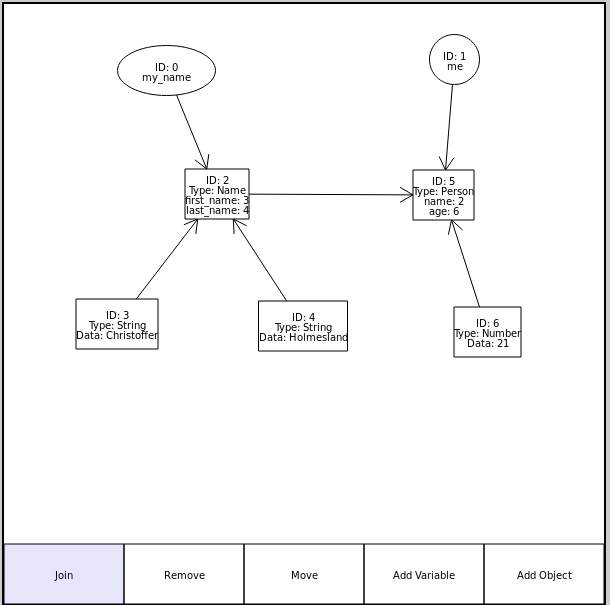
\includegraphics[width=0.75\linewidth]{/graphdrawer/pythonui}
    \caption{Python - user interface}
    \label{fig:graphdrawerPythonUserInterface}
\end{figure}
\noindent
The Python controller can work without any configuration, but it will only allow objects of the base types "String", "Number" and "Boolean". A configuration should, therefore, be supplied to allow for more engaging questions. The only configuration available is the \code{steps} property. The steps property should be an array with at least one element. When the Python interpreter is used, the last element in the array contains extra information about the classes and functions defined in the script. This step is examined for class information. Every defined class is added as an object type, and the code is parsed again to find the possible class properties.
\\[11pt]
Like the Graph0 controller, the Python controller implements different states and state handlers. The state can be changed by the user by clicking on one of the buttons "Join", "Remove", "Move", "Add Variable" or "Add Object". The join state lets the user define a relationship between a variable and object, or a relationship between two objects. The remove state lets the user remove a relationship or a node from the graph. The move state lets the user change the position of nodes. The Add Variable state asks the user for a variable name and lets them add it to the graph. The Add Object state asks the user for an object type, and optionally an object value if the object type is a value type, and lets them add it to the graph.
\\[11pt]
The variable and object concepts do not exist in the GraphDrawer; therefore they are defined in the controller. They are stored in the arrays \code{variables} and \code{objects}. A variable needs three properties, \code{name}, \code{links}, and \code{id}. \code{name} is a string with the name of the variable. \code{links} is an array where the elements are the objects which the variable references. \code{links} should never have more than one element, because a variable is only able to reference one object. It needs to be an array because the student is allowed to make mistakes. The \code{id} property is the identifier of the GraphDrawer node which is used to display the variable in the graph. The position of the node does not change the behavior of a variable, and it, therefore, does not need to store a complete copy of the node. This also makes converting a variable to JSON simpler, because there is only one node object.
\\[11pt]
An object needs several properties:
\begin{enumerate}
    \item \code{type}, which is a string determining the type of the object. E.g. \code{"String"}.
    \item \code{baseType}, is a boolean which is \code{true} if the \code{type} is either \code{"String"}, \code{"Number"} or \code{"Boolean"}.
    \item \code{value}, is used if the \code{baseType} is \code{true}. It contains the value of the object, e.g., \code{True}.
    \item \code{fields} is an array of field objects if the \code{baseType} is \code{false}. Field objects have two properties, \code{name} and \code{value}. The name is the name of the property, e.g., \code{"first\_name"}. The \code{value} is the id of the object containing the actual value of the property. This is done because if the object with the value is not a base type, then the value is another object. E.g., the \code{name} in the figure references an object of the Name class.
    \item \code{id}, which is the id of the GraphDrawer node used to display the object.
\end{enumerate}
To display meaningful information about variables and objects in the GraphDrawer nodes, the \code{generateNodeText} function should be used when a variable or object property changes. The text of GraphDrawer nodes needs to be a string in the \code{v} property. The function converts the properties to a string and adds it to the linked GraphDrawer node. Every node starts with text displaying the id of the node. This is done so the user can easily differentiate between two objects with the same values. The second line of a variable is the name of the variable. Object nodes also show the name of the properties defined in the \code{fields} array, and the id of the linked object. If the object does not have any fields, the object value is displayed instead. The resulting node text can be seen in the figure.
\\[11pt]
When the student answer is exported from the controller, it includes all the variables and objects created by the user. A copy of the complete GraphDrawer graph (nodes and edges) is also exported in case the student solution is not valid. When the solution is checked against the correct solution, the information about the variables and objects is used. When the solution is imported back into the GraphDrawer, the graph is used.
\\[11pt]
The process of importing the correct solution of a Python question is more complicated. The solution only contains information about the Python variables and objects. The controller objects and variables need to be created based on the given information. Only one step is read at a time, and this step is called "the solution". This process is however made simpler by the fact that the solution will always have the correct relationship defined between objects. The solution is imported by first creating controller variables from every variable in the solution. Every object in the solution will either be linked to by another object, or by a variable. It is, therefore, possible to import the solution objects, by starting at the list of objects linked to by the variables, and then recursively looking at any objects linked by the given objects. A combination of the \code{\_uniqueId} defined on GraphDrawer nodes, and the id reference on the solution objects are used to create the edges between the variables and objects.